\documentclass{article}
%
% Demo of the mcode package from 
% http://www.mathworks.co.uk/matlabcentral/fileexchange/8015-m-code-latex-package
% Updated 06 Mar 2014
%

% load package with ``framed'' and ``numbered'' option.
\usepackage[framed,numbered,autolinebreaks,useliterate]{mcode}

% something NOT relevant to the usage of the package.
\usepackage{url}
\usepackage{graphicx}

\setlength{\parindent}{0pt}
\setlength{\parskip}{18pt}
\title{\texttt{Sistemas de Control Inteligente \newline} Práctica 1. Identificación y control neuronal (III)}
\author{Pablo Acereda García y Laura Pérez Medeiro}
% //////////////////////////////////////////////////

\begin{document}

\maketitle

\section*{Identificación de un sistema usando una red NARX}

Usando el archivo proporcionado en la práctica, se crea un modelo usando ese sistema con una entrada aleatoria y almacenando las variables x e y en estructuras con tiempo, las cuales deben ser accesibles desde el Workspace. Para ello, se realizaran las siguientes configuraciones:


\begin{figure}[h]
\caption{Configuración para la entrada aleatoria}
\centering
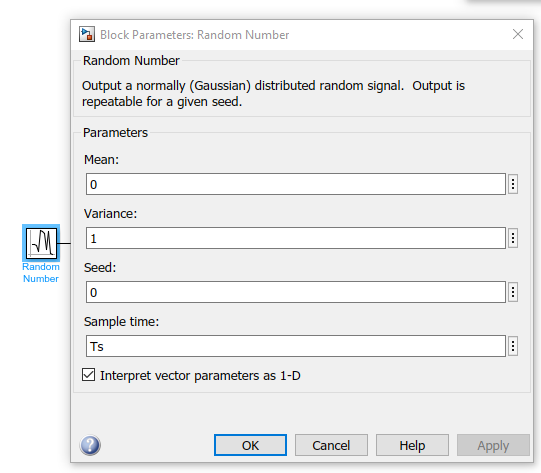
\includegraphics[width=0.5\textwidth]{imagenes/randomNumConf.png}
\end{figure}

\begin{figure}[h]
\caption{Configuración para la variable X, para que aparezca sin el formato out.X}
\centering
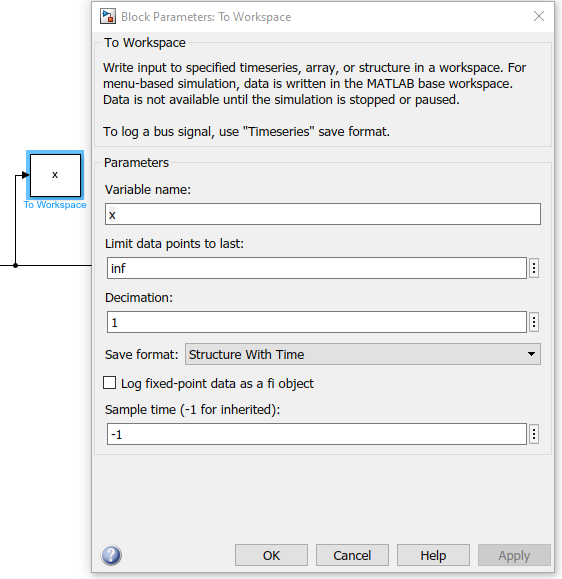
\includegraphics[width=0.5\textwidth]{imagenes/VarX.png}
\end{figure}

\begin{figure}[h]
\caption{Configuración para mostrar la variable en el área de trabajo de Matlab}
\centering
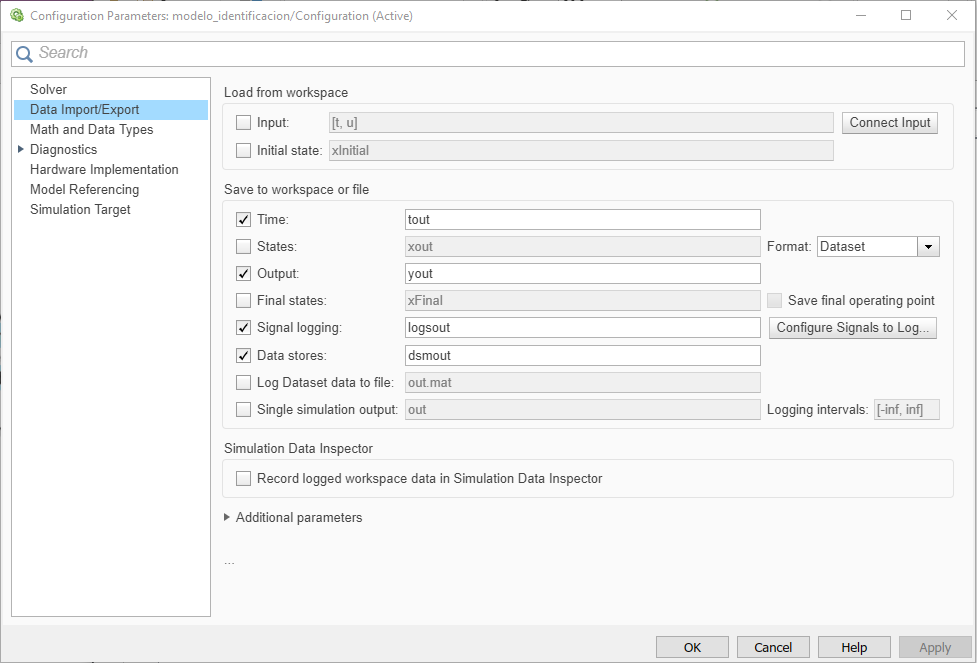
\includegraphics[width=0.5\textwidth]{imagenes/ConfigOut.png}
\end{figure}
\newpage
Mediante el siguiente código, el cual se encuentra en el archivo SimData.m, se generan los arrays de inputs y outputs:
\lstinputlisting{./Source/SimData.m}

A continuación se generará una red de tipo NARX con 5 neuronas en la capa oculta y dos retardos tanto en la entrada como la salida realimentada:
\lstinputlisting{./Source/NARX_NeuronalNetwork_1.m}

Finalmente, se genera un modelo de Simulink que contenga a la red entrenada mediante el comando: \mcode{gensim(net, Ts)}





















\section*{Usage --- 3 ways}

1) This inline demo \mcode{for i=1:3, disp('cool'); end;} uses the \verb|\mcode{}| command.\footnote{Works also in footnotes: \mcodefn{for i=1:3, disp('cool'); end;}}

2) The following is a block using the \verb|lstlisting| environment.
\begin{lstlisting}
for i = 1:3
	if i >= 5                    % literate programming replacement
		disp('cool');           % comment with some §\mcommentfont\LaTeX in it: $\mcommentfont\pi x^2$§
	end
	[~,ind] = max(vec);
	x_last = x(1,end);
	v(end);
	really really long really really long really really long really really long really really long line % blaaaaaaaa
end
\end{lstlisting}
Note: Here, the package was loaded with the \verb|framed|, \verb|numbered|, \verb|autolinebreaks| and \verb|useliterate| options.  \textbf{Please see the top of mcode.sty for a detailed explanation of these options.}


3) Finally, you can also directly include an external m-file from somewhere on your hard drive (the very code you use in \textsc{Matlab}, if you want) using the \verb|\lstinputlisting{/SOME/PATH/FILENAME.M}| command.  If you only want to include certain lines from that file (for instance to skip a header), you can use \verb|\lstinputlisting[firstline=6, lastline=15]{/SOME/PATH/FILENAME.M}|.

\medskip


Florian (\texttt{florian@knorn.org})

\begin{center}
\begin{minipage}{.75\linewidth}
	\color{red}{\hfill\textbf{NOTE --- BEFORE YOU START}\hfill\strut}

	All that this package does is to configure the \verb|listings| package for you. If anything is not working the way you want it, refer to the \verb|listings| documentation first and / or take a look at the \verb|mcode.sty| file itself, which is well documented internally.\\
	
	The \verb|listings| documentation can be accessed either by typing \verb|texdoc listings| into a command prompt on your system, or online:\\\scriptsize\url{http://mirrors.ctan.org/macros/latex/contrib/listings/listings.pdf}
	
\end{minipage}
\end{center}

\end{document}
